\documentclass[twocolumn]{scndocument}

\usepackage{import}
\usepackage{scn}
\usepackage{fancyhdr}
\usepackage{titlesec}
\usepackage{caption}
\usepackage{float}

\usepackage{graphicx} % Required for inserting images

\pagestyle{fancy}
\fancyhf{} 
\fancyfoot[C]{\textbf{\thepage}} 


\begin{document}

\setcounter{page}{222}

\begin{list}{\labelitemi}{\leftmargin=2.5em \itemsep = 0pt}
    \item[\hspace{1em}]resources, including study materials, assignments, and tests;
    \item the ability to receive feedback from the system and teachers to assess progress and correct the learning process.
\end{list}
\textbf{The main disadvantages of an intelligent tutoring system:}
\begin{itemize}[noitemsep]
    \item limited ability of the system to adapt to the specific needs of students with different backgrounds and learning abilities;
    \item lack of accuracy in identifying student errors and failures, which may lead to underestimation of their real abilities;
    \item necessity of constant updating of educational content and algorithms of the system in accordance with changes in the discipline program and teaching methods;
    \item limited opportunities to interact with students outside the learning environment, which can make it difficult to solve individual questions and problems.
\end{itemize}

One of the best known systems in problem solving is \textbf{WolframAlpha} [2]. This system can solve problems from various fields, including graph theory problems.

This system supports functions such as graph editing, basic graph operations, providing examples with known graphs, and searching for elements in a subgraph.

However, the disadvantages of WolframAlpha are that it cannot provide step-by-step solutions to problems, it has a special query language that not every user can understand, and it does not provide training tasks for users.

\textbf{ALEKS} is an intelligent tutoring system that provides a customizable program for teaching students in different subject areas, including discrete mathematics [3]. The system uses an approach based on passive learning theory, which allows hypothesizing about a student’s knowledge and determining the most effective learning path based on the student’s learning data.

The ALEKS system uses mathematical algorithms that are the basis of its knowledge base and artificial intelligence technology. The ALEKS knowledge base is a system of concepts and tasks that are interconnected and divided into levels of complexity. Each assignment has its own unique difficulty level, which is determined based on the student’s study data. This allows students to learn at their own pace and make the most efficient use of their time.

The disadvantages of this approach are its limited depth of understanding of topics and its inability to integrate with other systems. This can lead to limitations in using the system within broader programs of study and limitations in accessing deeper knowledge of discrete mathematics. In addition, a customizable curriculum may be less effective with students who already have a certain level of knowledge in discrete mathematics and do not require such customization.

\textbf{Webwork} is a system of online teaching materials [4]. This system allows teachers to create individual assignments and exercises that students can solve in real time, and also provides the ability to automatically create different versions of assignments and assessments, and use interactive elements such as graphs and visualizations to facilitate the understanding of the material.

The Webwork information base consists of mathematical formulas, algorithms for solving problems, and a database containing assignments and students’ answers. The Webwork approach allows new assignments and answers to be quickly added to the database, which is its advantage. However, the disadvantage is the limited functionality, since Webwork cannot use complex mathematical objects such as graphs or matrices. Also, dueto the lack of systematization and semantic structuring of knowledge, it is impossible to automate the process of creating tasks and generating answers, and in the absence of a certain problem in the database its solution will not be found.

\textbf{Maple T. A.} is a program that allows teachers to create and automatically check tests and assignments in discrete mathematics [5]. Maple T.A. uses a combination of several approaches. First, this system uses traditional mathematical methods to develop an information base, including the creation of test assignments and courses, and a semantic approach to create knowledge models and intelligent data processing systems. Second, it utilizes machine learning algorithms for adaptive learning and assessment of student knowledge, and incorporates automatic answer checking, manual evaluation, and proof checking. It is possible to add new mathematical objects such as graphs or matrices, which is an advantage of the system.

The system has limited functionality and no integration with other systems, which may limit its use in some areas. For example, in a business domain where it is important to have access to different systems and tools to solve problems, this limitation can be a significant disadvantage. In addition, the limited functionality may not meet the needs of users, which can lead to loss of interest and unproductive use of the system.

An intelligent tutoring system for discrete mathematics should not have the disadvantages inherent in the above systems, namely it should provide the ability to view step-by-step solutions, ease of integration with other systems, and ease of integrating new skills, knowledge, and themes into the existing system.

Also, the above systems are only able to solve a limited range of tasks that are predetermined by the developers, and the systems cannot generate tasks themselves for the user training.

\newpage

\titleformat{\section}{\centering\normalfont}{\Roman{section}.}{1em}{}

\setcounter{section}{1}
% \begin{center}
    \section{Proposed approach}
% \end{center}
The proposed approach implies the developing of a system based on the \textit{OSTIS Technology} and its basic principles to overcome these disadvantages [6].

\textit{OSTIS Technology} is a complex \textit{intelligent system} design technology based on semantic knowledge representation, which includes:
\begin{itemize}[noitemsep]
    \item library of generic, reusable and semantically compatible components and \textit{intelligent systems} (components of \textit{knowledge bases, intelligent problem solvers, intelligent user interfaces});
    \item compatible semantic knowledge representation languages of various kinds, providing semantic compatibility not only for reusable components of \textit{intelligent systems}, but also for entire \textit{intelligent systems};
    \item compatible semantic models of problem solving.
\end{itemize}

As a formal basis for knowledge representation within the framework of \textit{OSTIS technology}, a unified \textit{semantic network} with a set theory interpretation is used. Such a representation model is called \textit{SC-code} (Semantic computer code). The elements of such a \textit{semantic network} are called \textit{sc-nodes} and \textit{sc-connectors} (\textit{sc-arcs}, \textit{sc-edges}) [7]. A model of an entity described by means of \textit{SC-code} is called a \textit{sc-model}.

Intelligent systems developed with the use of the \textit{OSTIS Technology} are called \textit{ostis-systems}. Each \textit{ostis-system} consists of a platform-independent unified logicalsemantic model of this system (\textit{sc-model} of a computer system) and a platform for interpretation of such models. In turn, each \textit{sc-model} of a computer system can be decomposed into \textit{sc-model of a knowledge base, scmodel of a knowledge processing machine, sc-model of an interface} and \textit{an abstract sc-memory} where \textit{SC-code} constructions are stored [7].

The creation of \textit{sc-models of the knowledge base} is based on the ontological approach, which implies the creation of ontologies as systems of concepts describing a particular subject area [8].

The problem solver is the main part of the \textit{sc-model of the knowledge processing machine}, which is built on the basis of a \textit{multi-agent} approach, where the interaction of \textit{agents}, called \textit{sc-agents}, is carried out exclusively by means of \textit{semantic memory}, which stores \textit{SC-code} constructions [9]. This approach allows to ensure modularity and flexibility of the developed machine, and also provides the possibility of parallel execution of different knowledge processing processes.

\begin{center}
    \section{Knowledge base}
\end{center}

An important step in the design of \textit{intelligent tutoring systems for discrete mathematics} is the creation of a \textit{knowledge base} that will contain complete and structured information on \textit{discrete mathematics}. However, in order for this \textit{knowledge base} to be as useful and effective as possible, it is necessary to consider a number of criteria that will allow it to be evaluated.

\textbf{Based on this, the following basic and most important criteria for analyzing a knowledge base were
highlighted:}
\begin{itemize}[noitemsep]
    \item \textit{Knowledge base} for \textit{discrete mathematics} can be organized as a tree structure, where each node represents a particular topic, or as a network structure, where each node represents a different theorem or algorithm. Evaluating the structure of the \textit{knowledge base} may include analyzing the hierarchy of topics, the relationships between topics and individual elements of the \textit{knowledge base}, and the ease of navigating the \textit{knowledge base}.
    \item \textit{knowledge base} for \textit{discrete mathematics} should contain sufficient information about key concepts, theorems, algorithms, and applications. Assessment of the quality and completeness of the information may include verifying that all necessary definitions and theorems are present and that the information provided is accurate and reliable.
    \item \textit{knowledge base} for \textit{discrete mathematics} should be user-friendly and easily accessible for use by students, teachers and researchers. Evaluation of functionality and usability may include an analysis of the accessibility of the \textit{knowledge base} and the ability to search for information.
\end{itemize}

An important factor affecting the efficiency and quality of the system is the structured nature of the \textit{knowledge base}. For this purpose, it is necessary to have an organized hierarchy of partial \textit{subject domains}, which are strongly connected with each other by many different relations related to some common (base) \textit{subject domain}.

Figure 1 contains an example of the description of a \textbf{subject domain of graph theory}.

Determining the relations between concepts is an important step in the development of a \textit{knowledge base}, and requires careful analysis and careful approach. According to \textit{OSTIS Technology}, to achieve the best quality of the \textit{knowledge base}, concepts and relations will be described using their \textit{semantic neighborhoods}. The basic relations and concepts include identifier, definition, statement, inclusion and decomposition. The implementation of each relation and their representation in the \textit{knowledge base} depends on the particular case.

The next step is to define the rules and principles of describing the elements of the \textit{knowledge base}. If there are several concepts in the \textit{knowledge base} that are related to each other, the correct description of these concepts and connections between them allows to avoid duplication of information and ensure the integrity of the \textit{knowledge base}.

Figure 2 shows an example of the description of the concept \textbf{disconnected graph}.

\newpage

\captionsetup{labelsep=period} 

\begin{figure}[H]
    \centering
    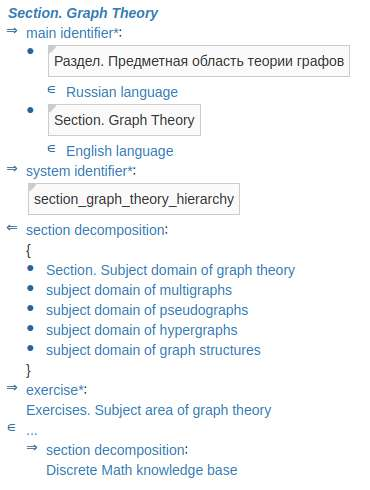
\includegraphics[width=0.9\linewidth]{1.jpg}
    \caption{Section. Subject domain of graph theory}
\end{figure}

\begin{figure}[H]
    \centering
    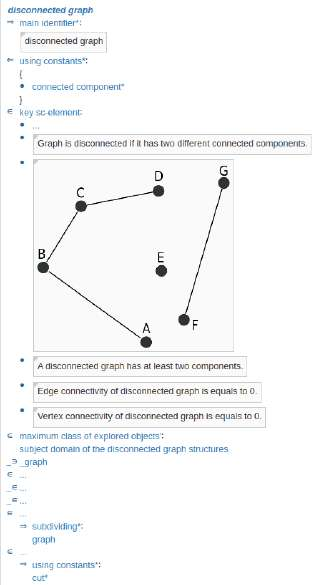
\includegraphics[width=0.9\linewidth]{2.jpg}
    \caption{Concept disconnected graph}
\end{figure}

\begin{figure}[H]
    \centering
    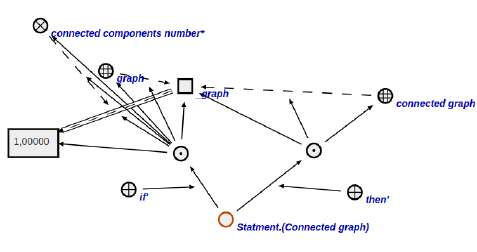
\includegraphics[width=0.9\linewidth]{3.jpg}
    \caption{Statement about connected graph}
\end{figure}

\begin{figure}[H]
    \centering
    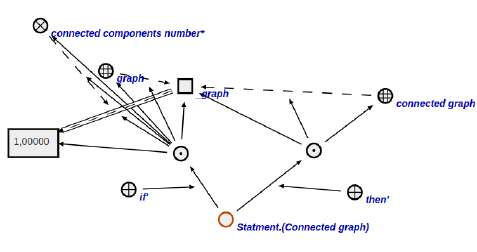
\includegraphics[width=0.9\linewidth]{3.jpg}
    \caption{Specification of program for finding the union of two graphs}
\end{figure}

\vspace{0.5cm}

A unified description of the elements of the \textit{knowledge base} creates an opportunity for its expansion in the future. The predefined rules and principles for describing elements will allow us to quickly and easily add new elements to the \textit{knowledge base} without having to redesign its entire structure. Thus, we can be sure that system is flexible and scalable [10].

An example of a statement about a \textit{connected graph} is shown in Figure 3, it is a logical formula written as an implication. The premise of the implication contains a pattern denoting that the graph has only one connectivity component. In the conclusion of the implication, the graph belongs to the set of connected graphs.

The \textit{knowledge base} also contains specifications of programs that can be used by the \textit{problem solver}. Thus, Figure 4 shows the specification of the \textit{graph union finding program}. The result of this program is a graph that is the union of two input graphs.

An example of an exercise is shown on Figure 5.
% \begin{center}
    \section {Problem solver}
% \end{center}
An important step in creating a \textit{intelligent tutoring system} for \textit{discrete mathematics} is to develop a \textit{problem solver} that will solve problems in \textit{discrete mathematics} with a full description of the step-by-step solution. But in order for the \textit{problem solver} to fully fulfill its function, it is necessary that the \textit{problem solver} meets the following criteria:

\end{document}